% !TEX root = morphkasten.tex

\section{Chassis}


%############## RAUPEN
\subsection{Raupen}

\begin{figure} [hbp]
	\centering
	\begin{subfigure}[b]{0.4\textwidth}
		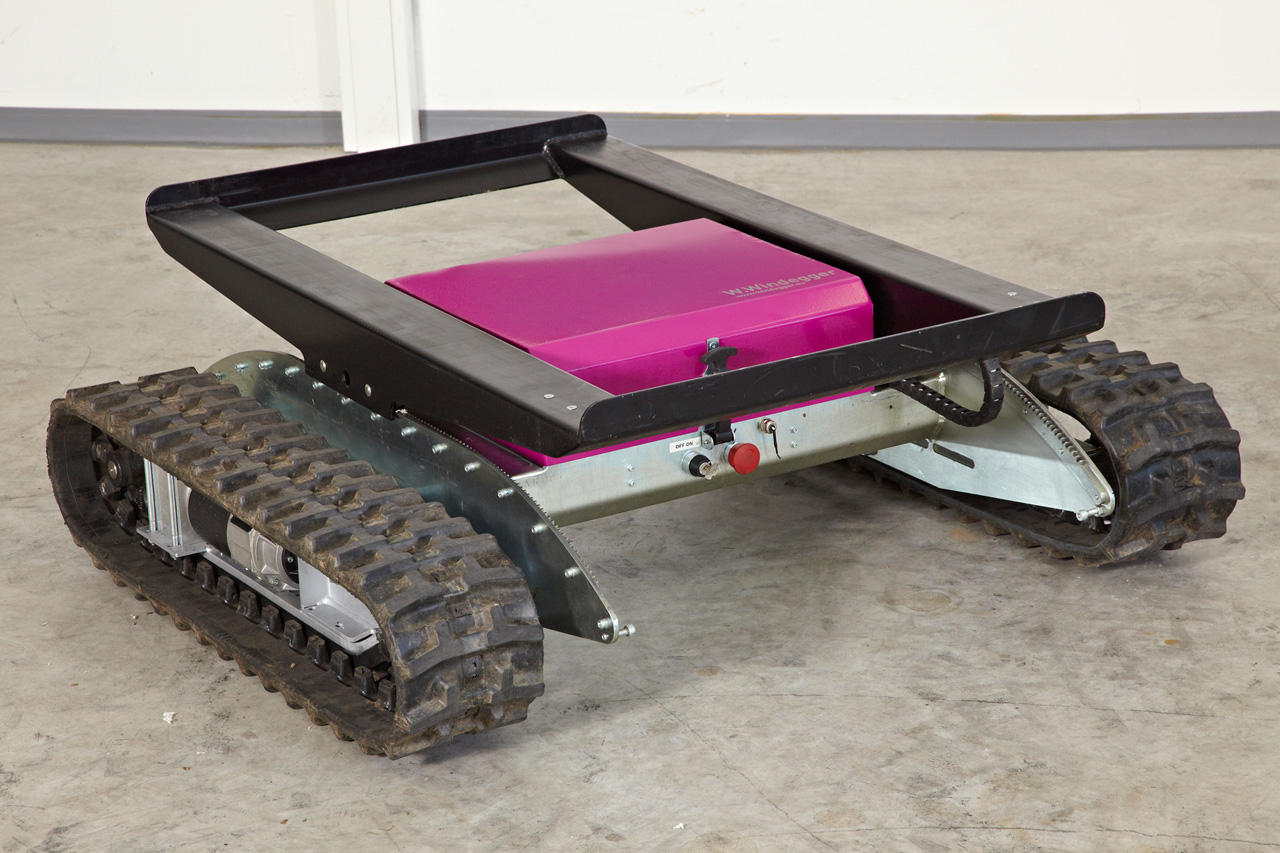
\includegraphics[width=\textwidth]{fig/Raupenfahrzeug.jpg}
		\caption{1.Situation: Modell 
		(Quelle: www.slowine-tech.de)}
	\end{subfigure}
	\hfill
	\begin{subfigure}[b]{0.36\textwidth}
		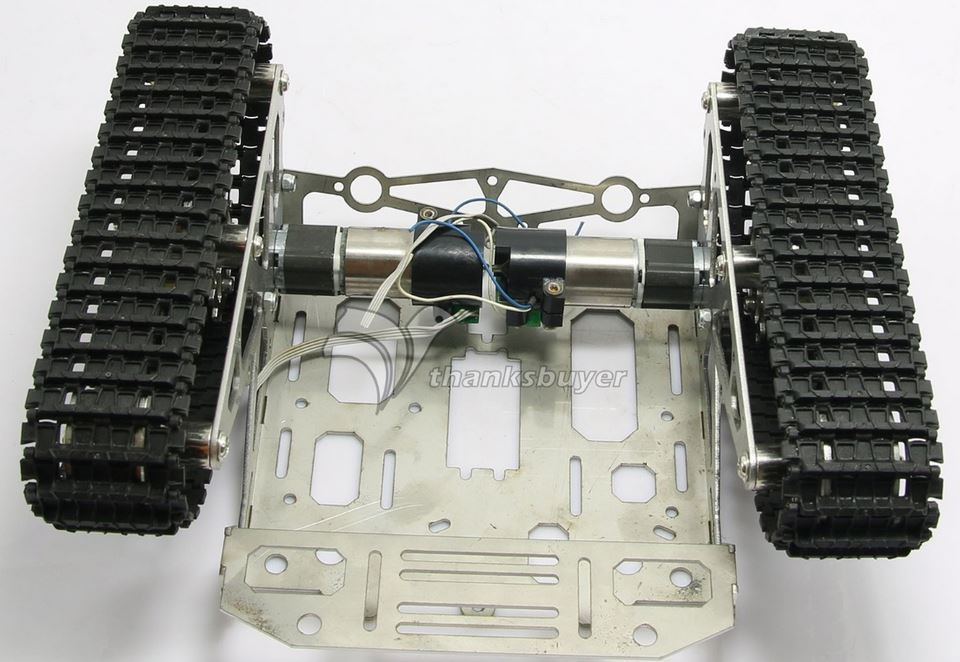
\includegraphics[width=\textwidth]{fig/Raupenfahrzeug-2.JPG}
		\caption{2. Situation: Ansicht von unten
		(Quelle: http://www.sainsmart.com/)}
\end{subfigure}
	\caption{Raupenfahrzeug}\label{fig:animals}
\end{figure}


\begin{table}[h]
\begin{tabular}{p{0.5\textwidth} | p{0.5\textwidth}}


 \textbf{Vorteile} & \textbf{Nachteile} \\ \hline
	 
\begin{itemize}
\item Lenkung sehr einfach Realisierbar
\item Technische Umsetzung einfach
\item Viele Beispiele im Internet verfügbar
\item Selbe Motoren für die Lenkung und den Antrieb
\end{itemize}

 
 &
 
\begin{itemize}
\item Verhalten bei Lenkung unklar
\item Längsämter als Räder
\item evtl. Schlupf zwischen Raupe und antrieb
\item eher für Geländefahrten geeignet
\item Drehpunkt der Lenkung in der Mitte der Raupen
\item gute Modellraupen sind teuer
\end{itemize}

\end{tabular}
\end{table}

\begin{table}[h]
\begin{tabular}{p{0.5\textwidth}p{0.5\textwidth}}


 \textbf{Risiken} & \\ \hline
	 
\begin{itemize}
\item Das verhalten beim Lenken ist unklar, somit kann es zu Fahrbahnabweichungen kommen.
\item Das finden von geeigneten Modellraupen mit unseren abmassen, könnte sich schwieg gestalten.
\end{itemize}
&
\begin{itemize}
\item Risiko 3
\item ...
\end{itemize}

 
\end{tabular}
\end{table}

\pagebreak


%############## 4-Rad Heckantrieb
\subsection{4-Rad Heckantrieb}

\begin{figure} [hbp]
	\centering
	\begin{subfigure}[b]{0.4\textwidth}
		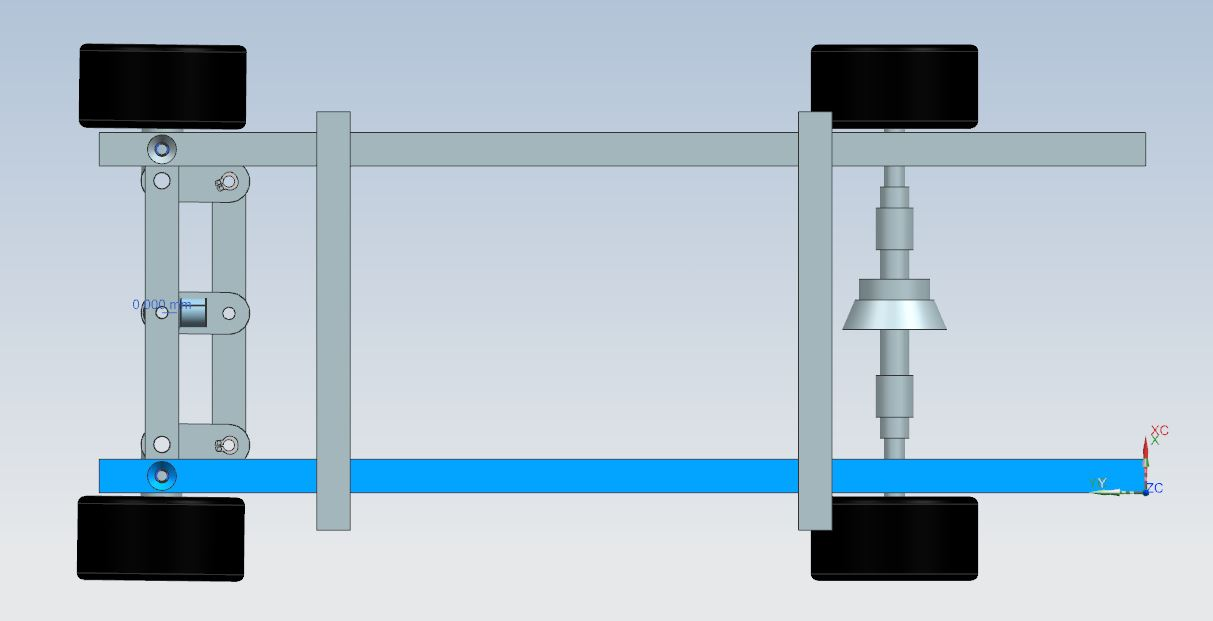
\includegraphics[width=\textwidth]{fig/4Rad-1.JPG}
		\caption{1.Situation: Ansicht von oben}
	\end{subfigure}
	\hfill
	\begin{subfigure}[b]{0.36\textwidth}
		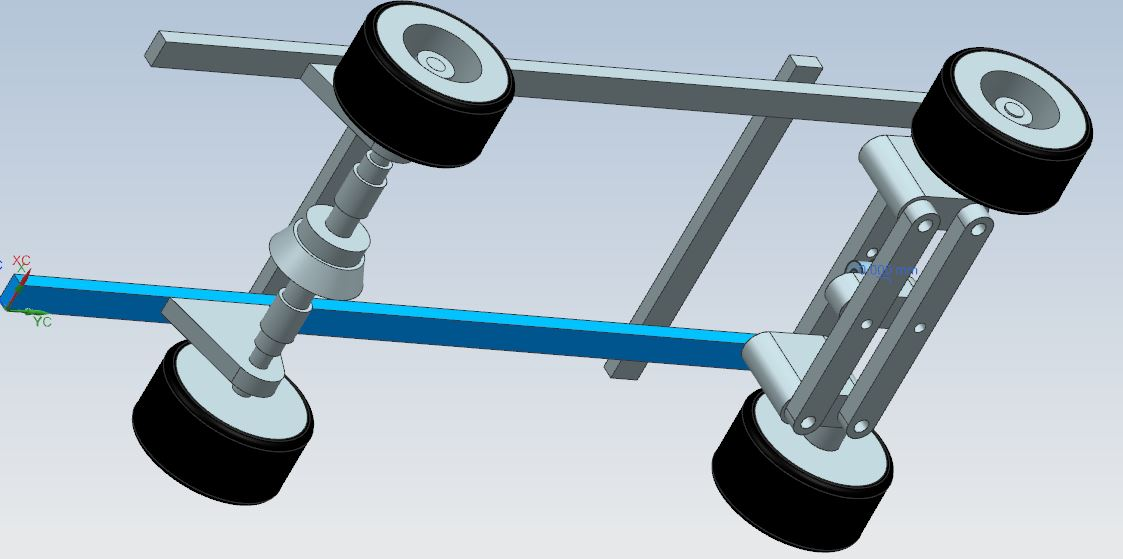
\includegraphics[width=\textwidth]{fig/4Rad-2.JPG}
		\caption{2. Situation: Ansicht von unten}
\end{subfigure}
	\caption{4-Rad mit Heckantrieb}\label{fig:animals}
\end{figure}

\begin{table}[h]
\begin{tabular}{p{0.5\textwidth} | p{0.5\textwidth}}


 \textbf{Vorteile} & \textbf{Nachteile} \\ \hline
	 
\begin{itemize}
\item Viel genutztes Prinzip im Modellbau
\item Viele Vorlagen im Internet
\item Klare Trennung zwischen Antrieb und Lenkung
\item sehr Stabil
\item 
\end{itemize}

 
 &
 
\begin{itemize}
\item Für den Heckantrieb ist ein Differential notwendig
\item Es muss eine Lenkung eingebaut werden 
\item Regelung der Lenkung ist aufwendig
\end{itemize}

\end{tabular}
\end{table}

\begin{table}[h]
\begin{tabular}{p{0.5\textwidth}p{0.5\textwidth}}


 \textbf{Risiken} & \\ \hline
	 
\begin{itemize}
\item Ist das Fahrzeug zu lang, könnte man in der Kurve mit den Hinterrädern die Fahrbahn verlassen.
\item Die Lenkung könnte zu unpräzise sein.
\end{itemize}
&
\begin{itemize}
\item Risiko 3
\item ...
\end{itemize}

 
\end{tabular}
\end{table}

\pagebreak


%############## 3-Rad
\subsection{3-Rad}

\begin{figure} [hbp]
	\centering
	\begin{subfigure}[b]{0.4\textwidth}
		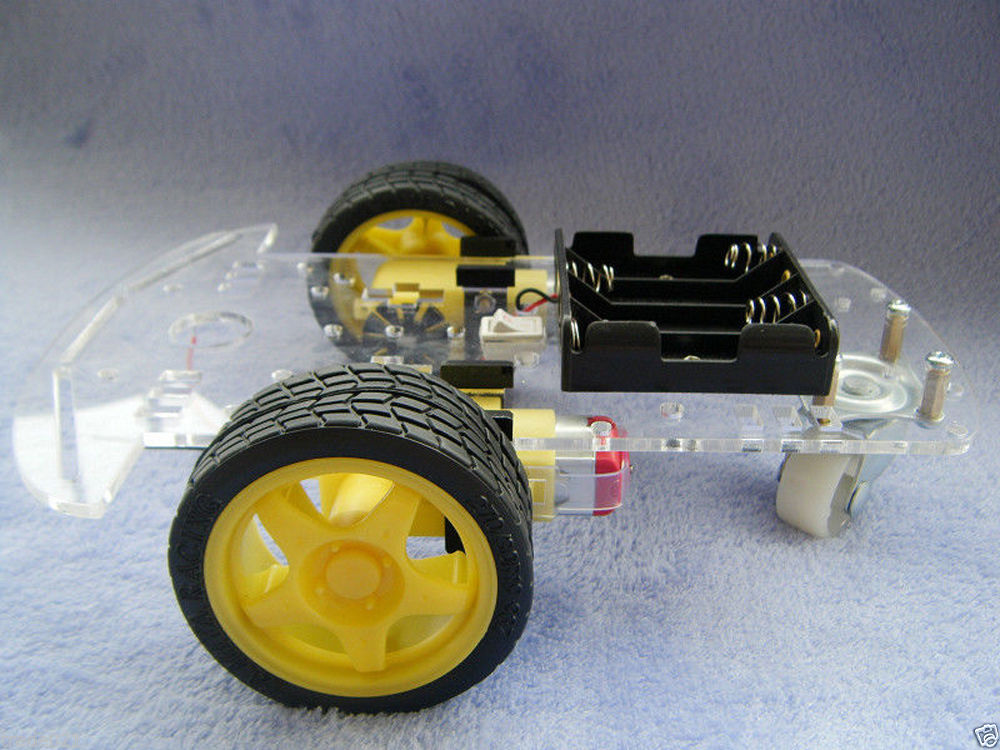
\includegraphics[width=\textwidth]{fig/3rad-1.jpg}
		\caption{1.Situation: Modell 
		(Quelle: www.sainsmart.com)}
	\end{subfigure}
	\hfill
	\begin{subfigure}[b]{0.36\textwidth}
		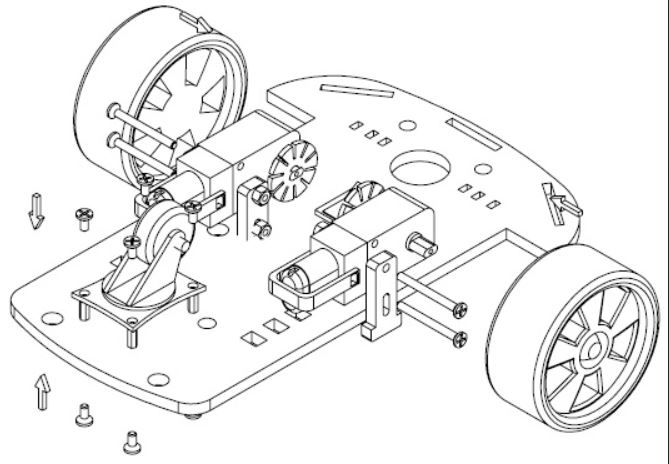
\includegraphics[width=\textwidth]{fig/3rad-3.JPG}
		\caption{2. Situation: Technische Zeichnung
		(Quelle: www.sainsmart.com)}
\end{subfigure}
	\caption{3-Rad Modell}\label{fig:animals}
\end{figure}

\begin{table}[h]
\begin{tabular}{p{0.5\textwidth} | p{0.5\textwidth}}


 \textbf{Vorteile} & \textbf{Nachteile} \\ \hline
	 
\begin{itemize}
\item Einfache Lenkung
\item Selber Motor für antrieb und Lenkung
\item sehr wendig
\item technisch einfach Realisierbar
\end{itemize}

 
 &
 
\begin{itemize}
\item Stabilität eher gering
\item Motoren müssen sehr genau sein
\item Grösse der Motoren für einen geeigneten antrieb 
\item Ausschlagen der Hinterachse
\end{itemize}

\end{tabular}
\end{table}

\begin{table}[h]
\begin{tabular}{p{0.5\textwidth}p{0.5\textwidth}}


 \textbf{Risiken} & \\ \hline
	 
\begin{itemize}
\item Bei einem 3-Rad Modell ist die Stabilität, dass grösste Problem. Beim aufladen des Containers könnte das Fahrzeug kippen.
\item Wenn die Antriebsräder in der Mitte montiert sind, braucht man Vorne und Hinten eine Stützrad oder eine Stützkugel. Diese könnten grössere Reibungskräfte verursachen.
\end{itemize}
&
\begin{itemize}
\item Risiko 3
\item ...
\end{itemize}

 
\end{tabular}
\end{table}

\pagebreak